% This is LLNCS.DEM the demonstration file of
% the LaTeX macro package from Springer-Verlag
% for Lecture Notes in Computer Science,
% version 2.4 for LaTeX2e as of 16. April 2010
%
\documentclass{llncs}
\usepackage{subfig}
\usepackage{graphicx}
%
\begin{document}
%
\frontmatter          % for the preliminaries
%
\pagestyle{headings}  % switches on printing of running heads
%
\mainmatter              % start of the contributions
%
\title{The use of Random Forest to predict binding affinity in docking}
%
\titlerunning{Mini Review on RF-Score}  % abbreviated title (for running head)
%                                     also used for the TOC unless
%                                     \toctitle is used
%
\author{Hongjian Li\inst{1} \and Kwong-Sak Leung\inst{1} \and Man-Hon Wong\inst{1} \and Pedro J. Ballester\inst{2}}
%
\authorrunning{Hongjian Li et al.} % abbreviated author list (for running head)
%
\institute{
Department of Computer Science and Engineering, Chinese University of Hong Kong, Sha Tin, New Territories, Hong Kong.\\
\and
Cancer Research Center of Marseille, INSERM U1068, F-13009 Marseille, France; Institut Paoli-Calmettes, F-13009 Marseille, France; Aix-Marseille Universit{\'e}, F-13284 Marseille, France; and CNRS UMR7258, F-13009 Marseille, France.\\
\email{pedro.ballester@inserm.fr}
}

\maketitle              % typeset the title of the contribution

\begin{abstract} % 70 to 150 words

Docking is a structure-based computational tool that can be used to predict the strength with which a small ligand molecule binds to a macromolecular target. Such binding affinity prediction is crucial to design molecules that bind more tightly to a target and thus are more likely to provide the most efficacious modulation of its biochemical function. Despite intense research over the years, improving this type of predictive accuracy has proven to be a very challenging task for any class of method.

New scoring functions based on non-parametric machine-learning regression models, which are able to exploit effectively much larger volumes of experimental data and circumvent the need for a predetermined functional form, have become the most accurate to predict binding affinity of diverse protein-ligand complexes. In this focused review, we describe the inception and further development of RF-Score \cite{564}, the first machine-learning scoring function to achieve a substantial improvement over classical scoring functions at binding affinity prediction. RF-Score employs Random Forest (RF) regression to relate a structural description of the complex with its binding affinity. The review will cover adequate benchmarking practices \cite{908}, studies exploring optimal intermolecular features \cite{1370}, further improvements \cite{1432} and RF-Score software availability including a user-friendly docking webserver \cite{1362} and a standalone executable for rescoring docked poses. Some work has also been made on the application of RF-Score to the related problem of virtual screening, e.g. a prospective virtual screening study \cite{1281}. This will be briefly discussed and the required future work outlined.

\keywords{molecular docking; scoring functions; random forest; chemical informatics; structural bioinformatics}

\end{abstract}

\section{Introduction}

Molecular docking is a key computational method in structure-based drug design, which has several important applications. First, given a X-ray crystal structure of a protein-ligand complex (e.g. Figure \ref{3NUX}), docking can identify 3D conformations of a known ligand that are conformationally close to the co-crystallised conformation (native pose identification). Second, docking can discriminate between known binders and non-binders with the goal of finding previously unknown binders in large databases of candidate molecules (virtual screening). Third, docking can predict the binding strength of known binders and their derivatives in order to identify more potent binders against the target (increasing potency) or less potent binders against an off-target (increasing selectivity).

\begin{figure}
\includegraphics[width=1.4\linewidth,natwidth=1400px,natheight=800px]{../rfscore3/3NUX.png}
\caption{Example of the X-ray crystal structure of a protein-ligand complex (PDB ID: 3NUX). The molecular surface of the protein is colored by secondary structure with 0.9 opacity to show the underlying secondary structure. The ligand molecule is pictured in stick representation colored by atom type. This figure was created by iview \cite{1366}, an interactive WebGL visualizer freely available at http://istar.cse.cuhk.edu.hk/iview/. iview does not require Java plugins, yet supports macromolecular surface construction and virtual reality effects.}
\label{3NUX}
\end{figure}

Operationally, docking predicts the position, orientation and conformation of a molecule when docked to the target's binding site (pose generation), as well as how tightly the docked pose of such putative ligand binds to the target (scoring). State-of-the-art docking programs such as AutoDock Vina \cite{595} and idock \cite{1153} perform reasonably well in pose generation and manage to obtain a redocking success rate of more than 50\% \cite{1362} on the common benchmarks of PDBbind v2012 and v2011 \cite{529,530} and the CSAR NRC HiQ Set 24Sept2010 \cite{857,960}. However, the single most critical limitation of docking is the low accuracy of the scoring functions that estimate the binding strength of a ligand. This binding affinity can thereafter be used to prioritize the molecules predicted to bind strongly for subsequent biological assays.

Classical scoring functions \cite{1313} assume a functional form relating a description of the crystal protein-ligand complex to its binding affinity, usually through Multiple Linear Regression (MLR). Non-parametric machine-learning scoring functions, on the other hand, circumvent the need of modelling assumptions implicit in functional forms, and have recently been demonstrated \cite{564,908} to introduce a substantial increase in the accuracy of scoring functions. 

In this review, we describe the inception and further development of RF-Score \cite{564}, the first machine-learning scoring function to achieve a large improvement over classical scoring functions \cite{1313} at binding affinity prediction. RF-Score employs Random Forest (RF) regression \cite{1309} to relate a structural description of the complex at atomic level with its binding affinity.

The review will cover adequate benchmarking practices, studies exploring optimal intermolecular features, further improvements and RF-Score software availability including a user-friendly docking webserver and a standalone executable for rescoring docked poses. Some work has also been made on the application of RF-Score to the related problem of virtual screening, e.g. a prospective virtual screening study. This will be briefly discussed and the required future work outlined. %TODO: rewrite.

\section{Random Forest (RF) scoring functions}

explain a bit of Random Forest, especially parts relevant to SFs such as mtry, etc. built a RF model with the 11 Vina features using the default number of trees (500). Instead of using all features, RF selects the best split at each node of the tree from a typically small number (mtry) of randomly chosen features. The mtry value with the lowest RMSE on Out-of-Bag (OOB) data is selected. %TODO: rewrote.

\subsection{RF-score}

RF-Score \cite{564}, the first scoring function using Random Forest (RF) \cite{1309} as the regression model, was found to outperform a range of widely-used classical scoring functions by a large margin.

RF-Score features are elemental occurrence counts of a set of protein-ligand atom pairs in a complex. To calculate these features, atom types were selected so as to generate features that are as dense as possible, while considering all the heavy atoms commonly observed in PDB complexes (C, N, O, F, P, S, Cl, Br, I). As the number of protein-ligand contacts is constant for a particular complex, the more atom types are considered, the sparser the resulting features will be. Therefore, a minimal set of atom types is selected by considering atomic number only. Furthermore, a smaller set of interaction features has the additional advantage of leading to computationally faster scoring functions.

RF-Score features are defined as the occurrence count of intermolecular contacts between elemental atom types $i$ and $j$, as shown in equations \ref{rfscore3:x_ij} and \ref{rfscore3:x}, where $d_{kl}$ is the Euclidean distance between the $k$th protein atom of type $j$ and the $l$th ligand atom of type $i$ calculated from a structure; $K_j$ is the total number of protein atoms of type $j$ ($\#\{j\}=9$) and $L_i$ is the total number of ligand atoms of type $i$ ($\#\{i\}=4$) in the considered complex; $\mathcal{H}$ is the Heaviside step function that counts contacts within a $d_{cutoff}$ neighbourhood. For example, $x_{7,8}$ is the number of occurrences of protein oxygen atoms hypothetically interacting with ligand nitrogen atoms within a chosen neighbourhood. This representation led to a total of 36 features. Therefore, each complex was characterized by a vector with 36 integer-valued features. Full details on RF-Score features are available at \cite{564,1295}.

\begin{equation}
\label{rfscore3:x_ij}
x_{ij}=\sum_{k=1}^{K_j}\sum_{l=1}^{L_i}\mathcal{H}(d_{cutoff}-d_{kl})
\end{equation}

\begin{equation}
\label{rfscore3:x}
\mathbf x=\{x_{ij}\}\in N^{36}
\end{equation}

As the number of protein-ligand contacts is constant for a particular complex, the more atom types are considered the sparser the resulting features will be. Therefore, a minimal set of atom types is selected by considering atomic number only. Furthermore, a smaller set of interaction features has the additional advantage of leading to computationally faster scoring functions. In this way, the features are defined as the occurrence count of intermolecular contacts between elemental atom types i and j:

\subsection{RF-Score-3}

RF-Score-3 is essentially RF-Score using a total of 47 features: the 36 RF-Score features \cite{564} in addition to the 6 AutoDock Vina features \cite{595}. Therefore, for a given random seed, a RF for each mtry value from 1 to 47 is built and that with the lowest RMSE on OOB data is selected as the scoring function.

\section{Experimental setup}

There are abundant examples of benchmarks to validate generic scoring functions \cite{1455,1456,571,1457}. Among them, the PDBbind benchmarks \cite{1313,1426} are arguably the most widely used for prediction of binding affinity of diverse complexes. Using a common and well-defined benchmark, where many scoring functions had been tested previously, has the advantage of minimising the risk of using a benchmark complementary to a particular scoring function.

\subsection{The PDBbind v2007 benchmark}

%Some figure here

Based on the 2007 version of the PDBbind database, it contains a particularly diverse collection of protein-ligand complexes from a systematic mining of the entire Protein Data Bank. This procedure led to a refined set of 1300 protein-ligand complexes along with their binding affinities. The PDBbind benchmark essentially consists of testing the predictions of scoring functions on the 2007 core set, which comprises 195 diverse complexes with measured binding affinities spanning more than 12 orders of magnitude, while using the remaining 1105 refined set complexes for training (i.e. both sets have no complexes in common). In this way, a set of protein-ligand complexes with measured binding affinity can be processed to give two non-overlapping data sets, where each complex is represented by its feature vector x(n) and its binding affinity y(n):

The v2007 benchmark contains a particularly diverse collection of 1300 protein-ligand complexes with their corresponding binding affinities, assembled through a systematic mining of the entire PDB (Protein Data Bank) \cite{540,537}.

The PDBbind benchmark essentially consists of testing the predictions of scoring functions on the 2007 core set, which comprises 195 diverse complexes with measured binding affinities spanning more than 12 orders of magnitude, while training in the remaining 1105 complexes in the refined set. In this way, a set of protein-ligand complexes with measured binding affinity can be processed to give two non-overlapping data sets, where each complex is represented by its feature vector $\mathbf x_i$ and its binding affinity $y_i$, which includes both pKd and pKi measurements, henceforth referred to as just pKd for simplicity:

\begin{equation}
\label{rfscore3:D_train}
D_{train}=\{y_i,\mathbf x_i\}_{i=1}^{1105}
\end{equation}

\begin{equation}
\label{rfscore3:D_test}
D_{test}=\{y_i,\mathbf x_i\}_{i=1106}^{1300}
\end{equation}

\begin{equation}
\label{rfscore3:y}
y=pK_d=-\log_{10}K_d
\end{equation}

\subsection{The 2013 blind benchmark}

A new benchmark mimicking a blind test has been recently proposed to provide a more realistic validation than the PDBbind benchmark, where higher performance is to be expected due to the protocol that generates this benchmark \cite{908}. The new test set comprises all the structures in the 2013 release of the PDBbind refined set that were not already in the 2012 release, i.e. the new protein-ligand complexes added in 2013, whereas the 2012 refined set is used for training. This is hence conducted as a blind test in that only data available until a certain year is used to build the scoring function that predicts the binding affinities of 2013 complexes as if these had not been measured yet. The PDBbind v2013 refined set (N=2959) and the PDBbind v2012 refined set (N=2897) have 2576 complexes in common. In the 2013 refined set, the 3rv4 protein consists of two Cs atoms which Vina does not support, so this complex was discarded. Eventually the test set has 2959-2576-1=382 complexes.

\subsection{Performance measures}

Predictive performance is quantified through commonly-used metrics \cite{1313}, including standard deviation SD in linear correlation, Pearson correlation coefficient Rp and Spearman correlation coefficient Rs between the measured and predicted binding affinities of the test set. The SD metric is essentially the residual standard error (RSE) metric used in some other studies \cite{963}.

The above three metrics are invariant under linear transformations, and are therefore for comparative purpose. In certain applications, the ultimate goal of a scoring function is to predict an absolute value of binding affinity as close to the measured value as possible. Hence the root mean square error RMSE between measured and predicted binding affinities without coupling a linear correlation constitutes a more realistic metric. Lower values in RMSE and SD and higher values in Rp and Rs imply better predictive performance.

Equations \ref{rmse}, \ref{sdev}, \ref{pcor} and \ref{scor} describe the mathematical expressions of the four metrics. Given a scoring function $f$ and the features $\mathbf{x}_i$ characterizing the $i$th complex out of $n$ complexes in the test set, $p_i=f(\mathbf{x}_i)$ is the predicted binding affinity, $\{\hat{p}_i\}_{i=1}^n$ are the fitted values from the linear model between $\{y_i\}_{i=1}^n$ and $\{p_i\}_{i=1}^n$ on the test set, whereas $\{y^r_i\}_{i=1}^n$ and $\{p^r_i\}_{i=1}^n$ are the rankings of $\{y_i\}_{i=1}^n$ and $\{p_i\}_{i=1}^n$, respectively.

\begin{equation}
RMSE=\sqrt{\frac{1}{n}\sum_{i=1}^n(p_i-y_i)^2}
\label{rmse}
\end{equation}

\begin{equation}
SD=\sqrt{\frac{1}{n-2}\sum_{i=1}^n(\hat{p}_i-y_i)^2}
\label{sdev}
\end{equation}

\begin{equation}
R_p=\frac{n\sum_{i=1}^np_iy_i-\sum_{i=1}^np_i\sum_{i=1}^ny_i}{\sqrt{(n\sum_{i=1}^n(p_i)^2-(\sum_{i=1}^np_i)^2)(n\sum_{i=1}^n(y_i)^2-(\sum_{i=1}^ny_i)^2)}}
\label{pcor}
\end{equation}

\begin{equation}
R_s=\frac{n\sum_{i=1}^np^r_iy^r_i-\sum_{i=1}^np^r_i\sum_{i=1}^ny^r_i}{\sqrt{(n\sum_{i=1}^n(p^r_i)^2-(\sum_{i=1}^np^r_i)^2)(n\sum_{i=1}^n(y^r_i)^2-(\sum_{i=1}^ny^r_i)^2)}}
\label{scor}
\end{equation}

\section{Results and discussion}

\subsection{RF-Score}

RF-Score \cite{564}, the first scoring function using Random Forest (RF) \cite{1309} as the regression model, was found to outperform a range of widely-used classical scoring functions by a large margin.

\subsection{SFC-ScoreRF}

I commented this SF in \cite{1370}

\subsection{RF-Score-2}

\cite{1370}

\subsection{RF-Score-3}

Main results from molecular informatics paper summarised here.

RF-Score-3 constitutes a remarkable improvement on the key requirement of predicting binding affinity when re-scoring redocked poses. Figure \ref{partition1+5stat}

\begin{figure}
\subfloat
{
  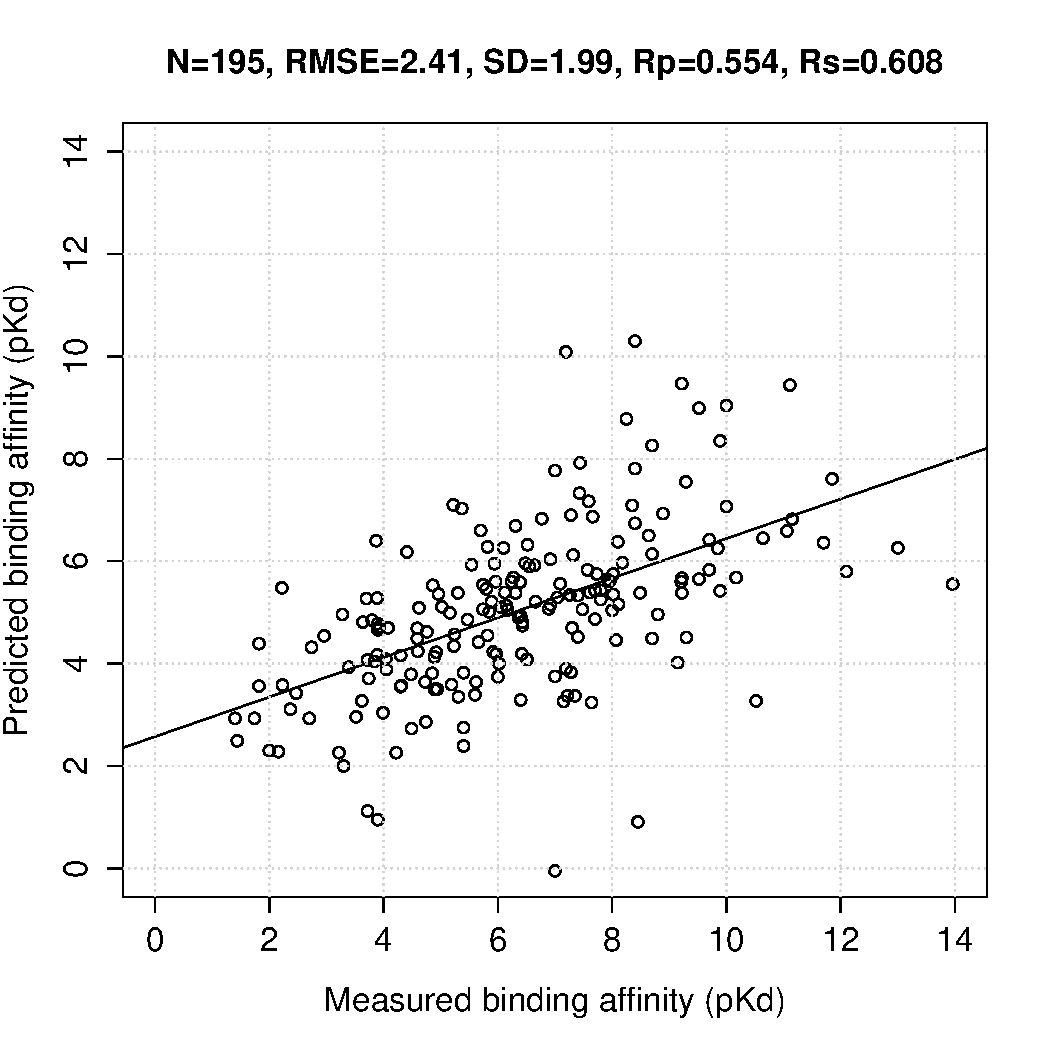
\includegraphics[width=0.48\linewidth]{../rfscore3/model-1-set-1-pdbbind-2007-tst-yp.eps}
}
\subfloat
{
  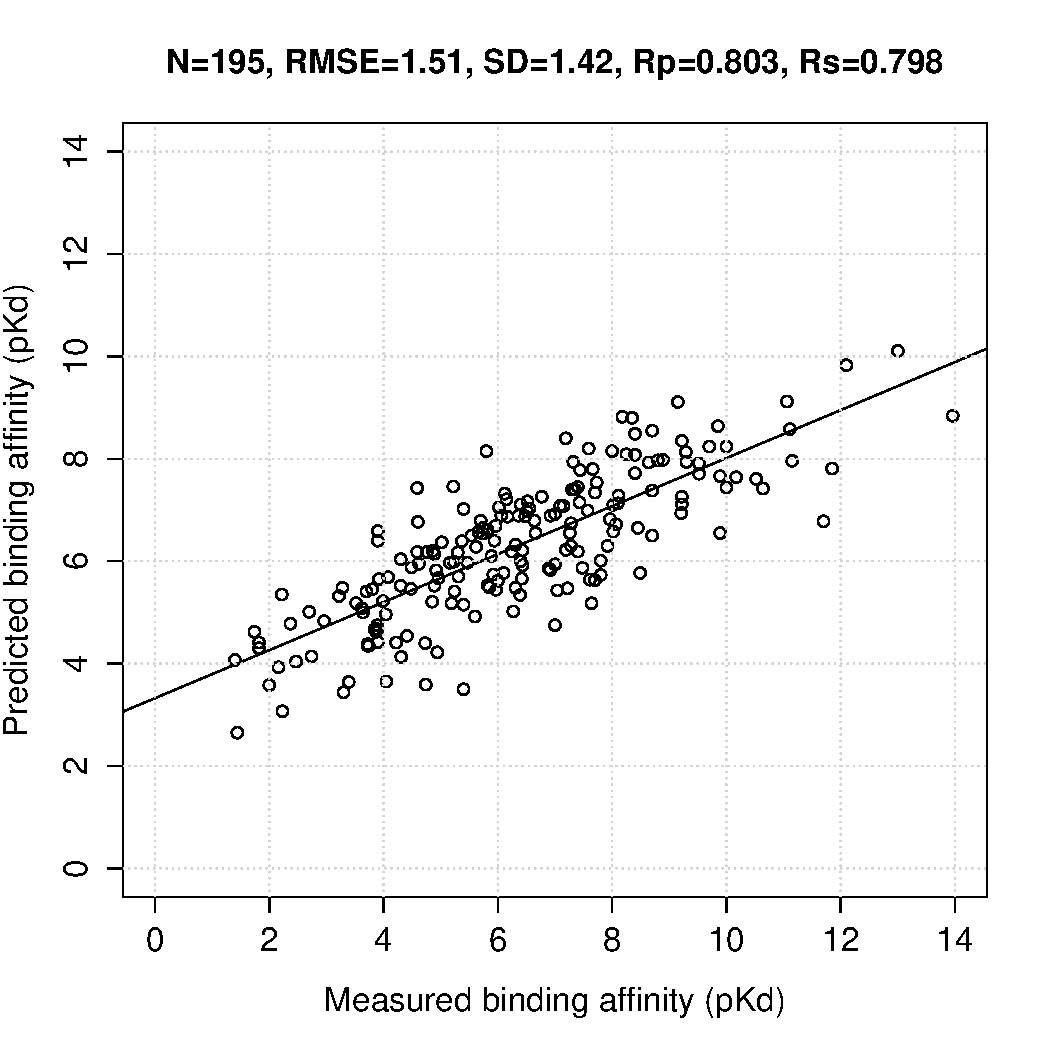
\includegraphics[width=0.48\linewidth]{../rfscore3/model-4-set-1-pdbbind-2007-tst-yp.eps}
}
\\
\subfloat
{
  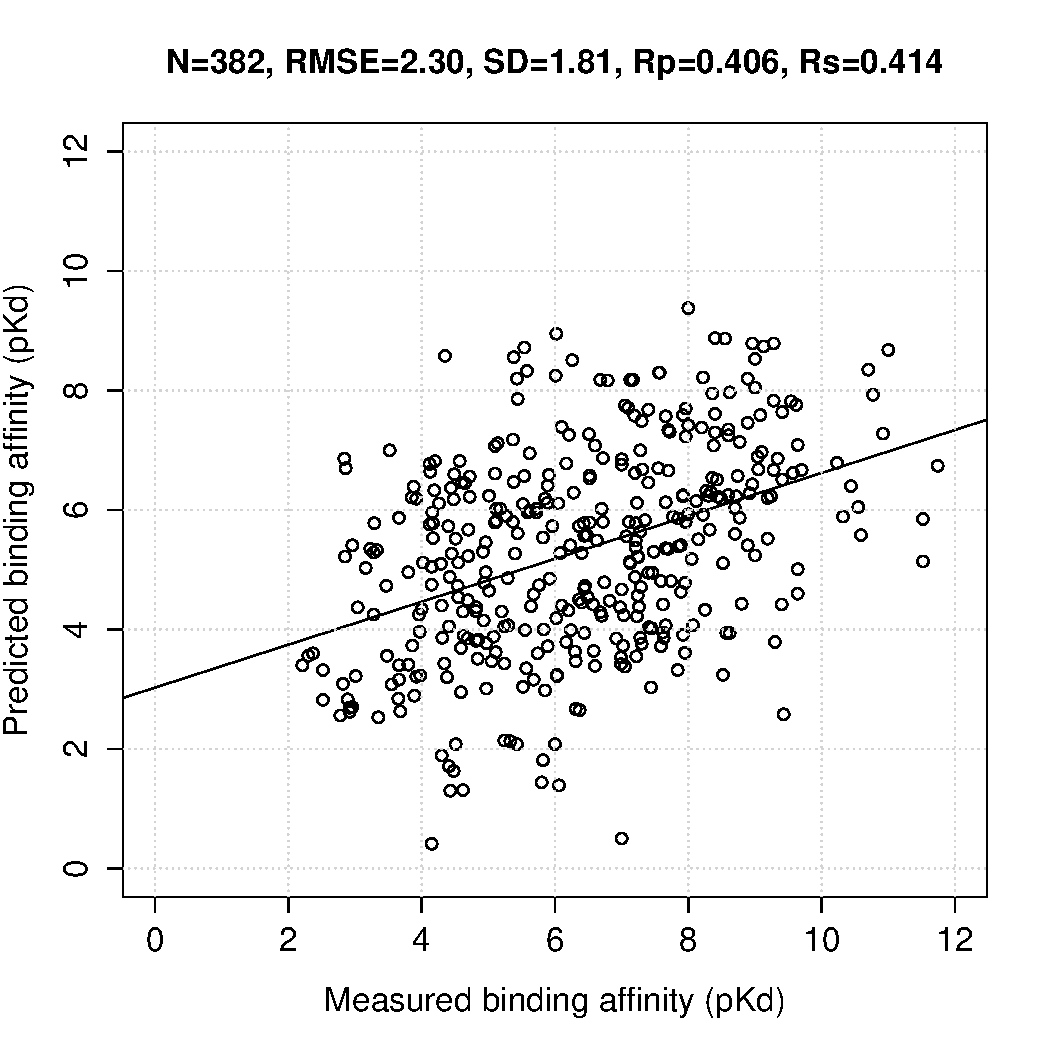
\includegraphics[width=0.48\linewidth]{../rfscore3/model-1-set-2-pdbbind-2007-tst-yp.eps}
}
\subfloat
{
  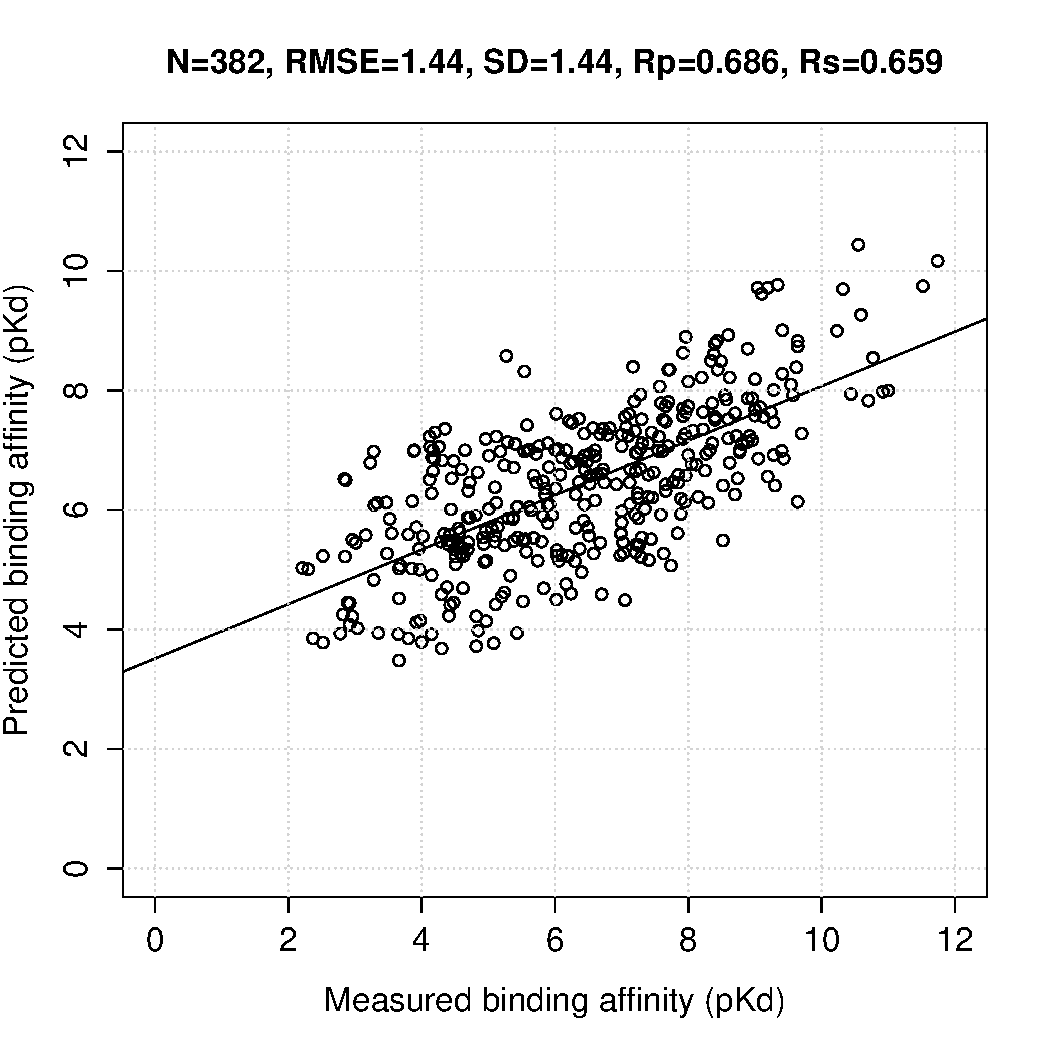
\includegraphics[width=0.48\linewidth]{../rfscore3/model-4-set-2-pdbbind-2012-tst-yp.eps}
}
\caption{Predictive performance of AutoDock Vina (left) and RF-Score-3 (right) on the PDBbind v2007 benchmark (top) and the PDBbind v2013 blind benchmark (bottom).}
\label{partition1+5stat}
\end{figure}

Table \ref{trn1105tst195} compares the performance of 25 scoring functions. Notably, the top 4 are all RF scoring functions.

\begin{table}
\caption{Predictive performance of 23 scoring functions evaluated on PDBbind v2007 benchmark.}
\label{trn1105tst195}
\begin{tabular}{lrrr}
\hline
Scoring function & Rp & Rs & SD\\
\hline
RF-Score-3       & 0.803 & 0.798 & 1.42\\
RF-Score-2       & 0.803 & 0.797 & 1.54\\
SFCscoreRF       & 0.779 & 0.788 & 1.56\\
RF-Score         & 0.774 & 0.762 & 1.59\\
ID-Score         & 0.753 & 0.779 & 1.63\\
SVR-Score        & 0.726 & 0.739 & 1.70\\
Cyscore          & 0.660 & 0.687 & 1.79\\
X-Score::HMScore & 0.644 & 0.705 & 1.83\\
DrugScoreCSD     & 0.569 & 0.627 & 1.96\\
SYBYL::ChemScore & 0.555 & 0.585 & 1.98\\
DS::PLP1         & 0.545 & 0.588 & 2.00\\
GOLD::ASP        & 0.534 & 0.577 & 2.02\\
SYBYL::G-Score   & 0.492 & 0.536 & 2.08\\
DS::LUDI3        & 0.487 & 0.478 & 2.09\\
DS::LigScore2    & 0.464 & 0.507 & 2.12\\
GlideScore-XP    & 0.457 & 0.435 & 2.14\\
DS::PMF          & 0.445 & 0.448 & 2.14\\
GOLD::ChemScore  & 0.441 & 0.452 & 2.15\\
SYBYL::D-Score   & 0.392 & 0.447 & 2.19\\
DS::Jain         & 0.316 & 0.346 & 2.24\\
GOLD::GoldScore  & 0.295 & 0.322 & 2.29\\
SYBYL::PMF-Score & 0.268 & 0.273 & 2.29\\
SYBYL::F-Score   & 0.216 & 0.243 & 2.35\\
\hline
\end{tabular}
\end{table}

%CIBB 3 \cite{1433}
%CIBB 4 \cite{1434}

\subsection{RF for virtual screening}

RF-Score has recently been used \cite{1281} to discover a large number of innovative binders of antibacterial targets and has now been incorporated \cite{1362} into a large-scale docking tool for prospective virtual screening (http://istar.cse.cuhk.edu.hk/idock/). To avoid confounding factors introduced by pose generation, these studies on scoring accuracy are carried out on data consisting of large sets of X-ray structures of protein-ligand complexes. However, scoring of the docked poses of a molecule is required in those cases where the experimentally-determined pose is not available.

With binary classifiers, not SF, one work showing RF promising (i.e. better than classical SFs also in this application): \cite{1632}

In the future, retrospective virtual screening (stress another application).

\subsection{Conclusions and Future Prospects}

Not too long, perhaps mentioning that what we will do next is important.

\section{Acknowledgements}

This work has been carried out thanks to the support of the A*MIDEX grant (n$^\circ$ ANR-11-IDEX-0001-02) funded by the French Government $\ll$ Investissements d'Avenir $\gg$ program, the Direct Grant from the Chinese University of Hong Kong and the GRF Grant (Project Reference 414413) from the Research Grants Council of Hong Kong SAR.

3.	1295 LNCS
10.	596 AutoDock4
11.	597 AutoDock
12.	595 AutoDock Vina

\bibliographystyle{splncs03}
\bibliography{../refworks}

\end{document}
